\documentclass[11pt,a4paper]{article}

\usepackage[T1]{fontenc}
\usepackage[utf8]{inputenc}
\usepackage{lmodern}
\usepackage{amsmath}
\usepackage[a4paper,margin=24mm]{geometry}
\usepackage{booktabs}
\usepackage{graphicx}
\usepackage{float}
\usepackage{caption}
\usepackage{enumitem}
\captionsetup{font=small,labelfont=bf,skip=6pt}
\setlist{nosep,leftmargin=1.4em}
\graphicspath{{assets/}}
\setlength{\parskip}{0.4\baselineskip}
\setlength{\parindent}{0pt}
\frenchspacing

\title{\vspace{-8mm}BeSecured: a local cybersecurity risk scanner\\[3pt]
  \large P12 progress report, week 8 of 10}
\author{Mohammedreda El Aroui (project manager), Sidi Hamadi,\\
  Philemon Vittet, Abdelrahmn Dahy}
\date{21 June 2026}

\begin{document}
\maketitle

BeSecured looks at the security settings of a personal computer and turns them into a
score out of 100, with a short list of things to fix. It is meant for people who are
not security experts. This note says where we are at week 8 of 10, and what was built
since the previous report.

\section{Where we are}

The hard part is done. The scanner runs on Windows, macOS and Linux, the score is
computed and explained, and the interface works locally from start to finish. Weeks 1
to 7 are finished. Week 8, the current one, is mostly packaging and tests: getting the
app to open with a double click, and closing the last gaps in the test suite. The two
remaining weeks are kept for the optional plain-language explanations and the final
delivery.

\begin{table}[h]
\centering\small
\begin{tabular}{@{}cll@{}}
\toprule
Week & Focus & State \\
\midrule
1--4 & Charter, planning, design, environment & done \\
5 & Cross-platform scanner & done \\
6 & Scoring engine & done \\
7 & Local interface and report export & done \\
8 & Packaging and tests & in progress \\
9--10 & Optional AI explanations, final delivery & to do \\
\bottomrule
\end{tabular}
\end{table}

One thing changed since the previous report. We had planned a React and Tailwind front
end with Chart.js. In the end we dropped all of that. The tool is now a plain Python
package with no external dependency, and the interface is hand-written HTML and CSS
served locally. For a tool whose whole point is to stay on the machine, fewer moving
parts is the right trade.

\section{What we built}

We started from a PowerShell script that only worked on Windows. It is now a Python
package. A single entry point runs the checks that apply to any system, then the ones
specific to the current operating system, collects the findings, and computes the
score. The interface is served by a small local server that talks to the scanner
through one local endpoint.

\begin{table}[h]
\centering\small
\begin{tabular}{@{}ll@{}}
\toprule
Module & Responsibility \\
\midrule
\texttt{scanner.py} & Entry point: runs the checks, dispatches by OS, builds the result. \\
\texttt{checks/common.py} & System info, privileges, listening ports. \\
\texttt{checks/windows.py} & Firewall, Defender, updates, users, policy, shares, startup, UAC, BitLocker. \\
\texttt{checks/macos.py} & Firewall, FileVault, Gatekeeper, SIP, XProtect, sharing, login items. \\
\texttt{checks/linux.py} & Firewall, updates, LUKS, users, password rules, shares, startup, antivirus. \\
\texttt{models.py} & Finding and result data, with a stable JSON shape. \\
\texttt{scoring.py} & Score, grade, per-category and per-finding impact. \\
\texttt{report.py} & HTML and JSON export. \\
\texttt{ui/} & Local server and browser interface. \\
\bottomrule
\end{tabular}
\end{table}

Each operating system has its own module, but the categories line up so the score
reads the same way everywhere. The table below lists what each scan looks at.

\begin{table}[h]
\centering\small
\begin{tabular}{@{}lll@{}}
\toprule
Area & What it reads & Platforms \\
\midrule
Open ports & Listening TCP ports and risky services (RDP, SMB, SSH, VNC) & all \\
Firewall & Local firewall state and profiles & all \\
Updates & Freshness of system and software updates & all \\
Accounts & Administrators, guest access, accounts without a password & all \\
Password policy & Minimum length and expiry, where readable & Win, Linux \\
Shared folders & SMB, NFS or non-standard system shares & all \\
Startup programs & Startup entries, with temporary paths flagged & all \\
Protection & Antivirus or native protection and signature freshness & all \\
Disk encryption & BitLocker, FileVault or LUKS state & all \\
Hardening & UAC on Windows, Gatekeeper and SIP on macOS & Win, macOS \\
\bottomrule
\end{tabular}
\end{table}

This sprint we hardened the parsing of each check. The output of system tools varies a
lot between machines and versions, so a parser that assumes a fixed format breaks
easily. Now a malformed or missing output becomes a skipped check with a short note,
not a crash. That work is most of the reason the test count grew this sprint.

\subsection*{Scoring}

A check ends as OK, a warning, or critical; a few are marked info or skipped. Only the
first three move the score. A warning costs 2 points, a critical one costs 5, and the
final score is 100 minus the share of points lost.
\[
\text{score} = 100 - \operatorname{round}\!\left(\frac{\text{points lost}}{\text{points possible}} \times 100\right)
\]
A skipped check, for example one that needs administrator rights we do not have, is
shown as skipped and never counted as a pass. We would rather show a gap than hide it.
The grade follows the score: A from 90, B from 75, C from 60, D from 40, F below.

\section{The interface}

The interface opens in its own window, without a browser address bar, so it reads like
a small system tool rather than a web page. It has five screens: a home screen to start
the scan and see what gets checked, an overview with the score, a list of categories, a
list of issues to fix, and a report screen to export the result. Each finding states
what was seen, why it matters, and the steps to fix it (Figures~\ref{fig:home}
and~\ref{fig:issues}).

\begin{figure}[H]
\centering
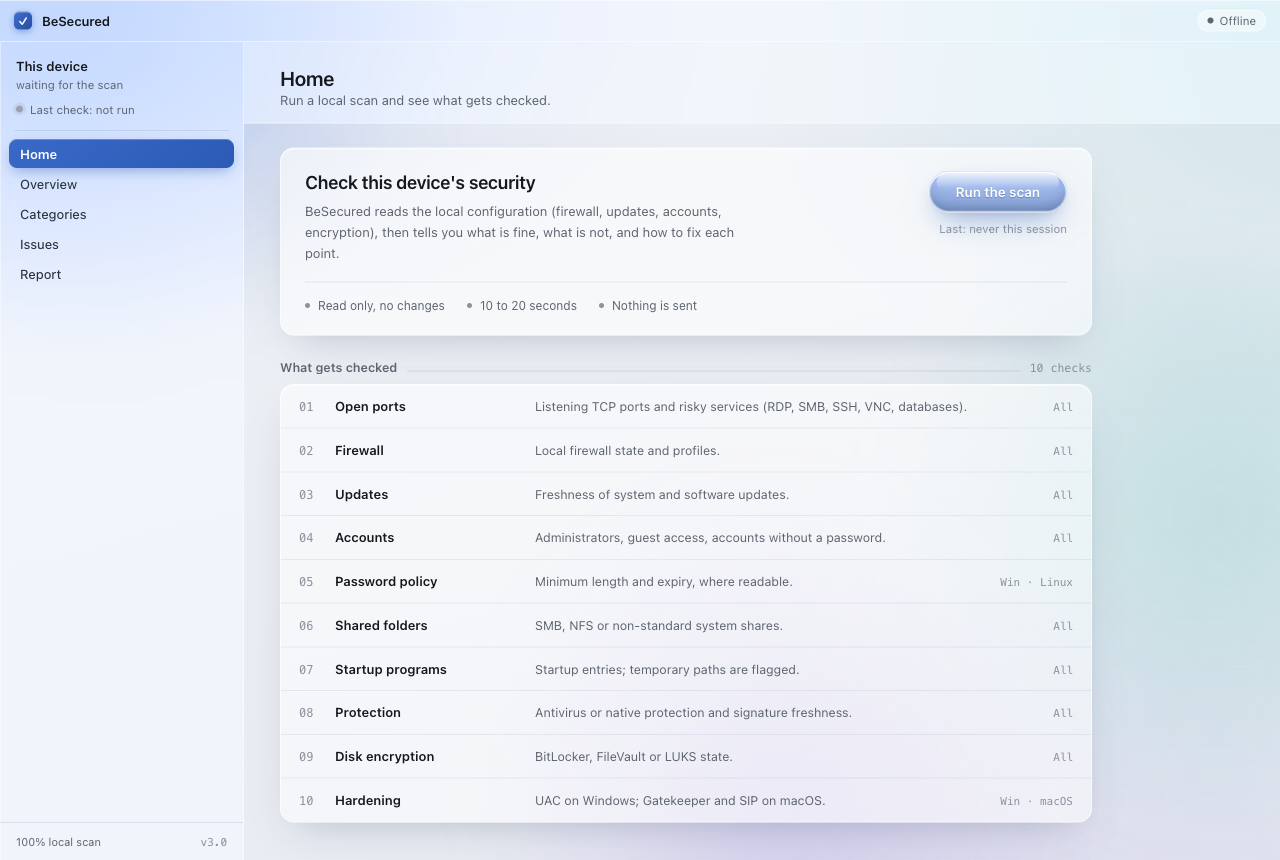
\includegraphics[width=0.82\linewidth]{ui-home.png}
\caption{Home screen: one action to start, and the list of what the scan reads. The
window opens in its own frame, without a browser address bar.}
\label{fig:home}
\end{figure}

The colours and the motion are not improvised. Every text colour clears the WCAG AA
contrast bar of 4.5 to 1 on white, and severity is never shown by colour alone: each
finding carries a colour, an icon and a label, because about one man in twelve cannot
tell red from green. Motion is kept to a few short transitions and respects the system
reduced-motion setting. The reasoning is written down in two short research notes kept
in the repository, one on colour and contrast, one on motion, so the look is a
deliberate choice rather than a default.

\begin{figure}[H]
\centering
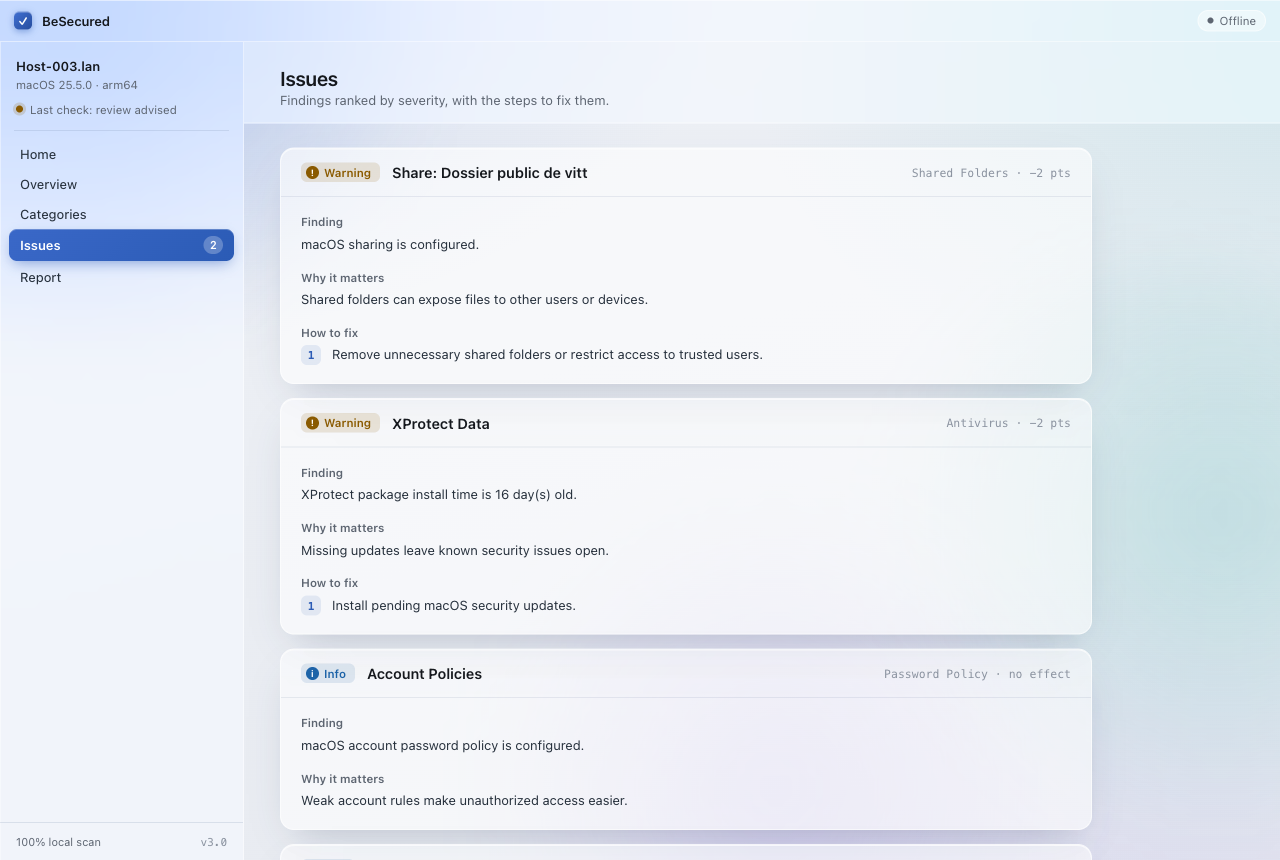
\includegraphics[width=0.82\linewidth]{ui-issues.png}
\caption{Issues, ranked by severity. Severity is shown by colour, an icon and a label
at once, so it stays readable for colour-blind users.}
\label{fig:issues}
\end{figure}

\section{A real scan}

Figure~\ref{fig:overview} is a scan run on one of our macOS machines. It scored 92 out
of 100, grade A. No critical issue, two warnings (an XProtect signature a couple of
weeks old, and a public shared folder), and the rest fine. The overview shows the
score, the breakdown by status, and the two warnings as top priority.

\begin{figure}[H]
\centering
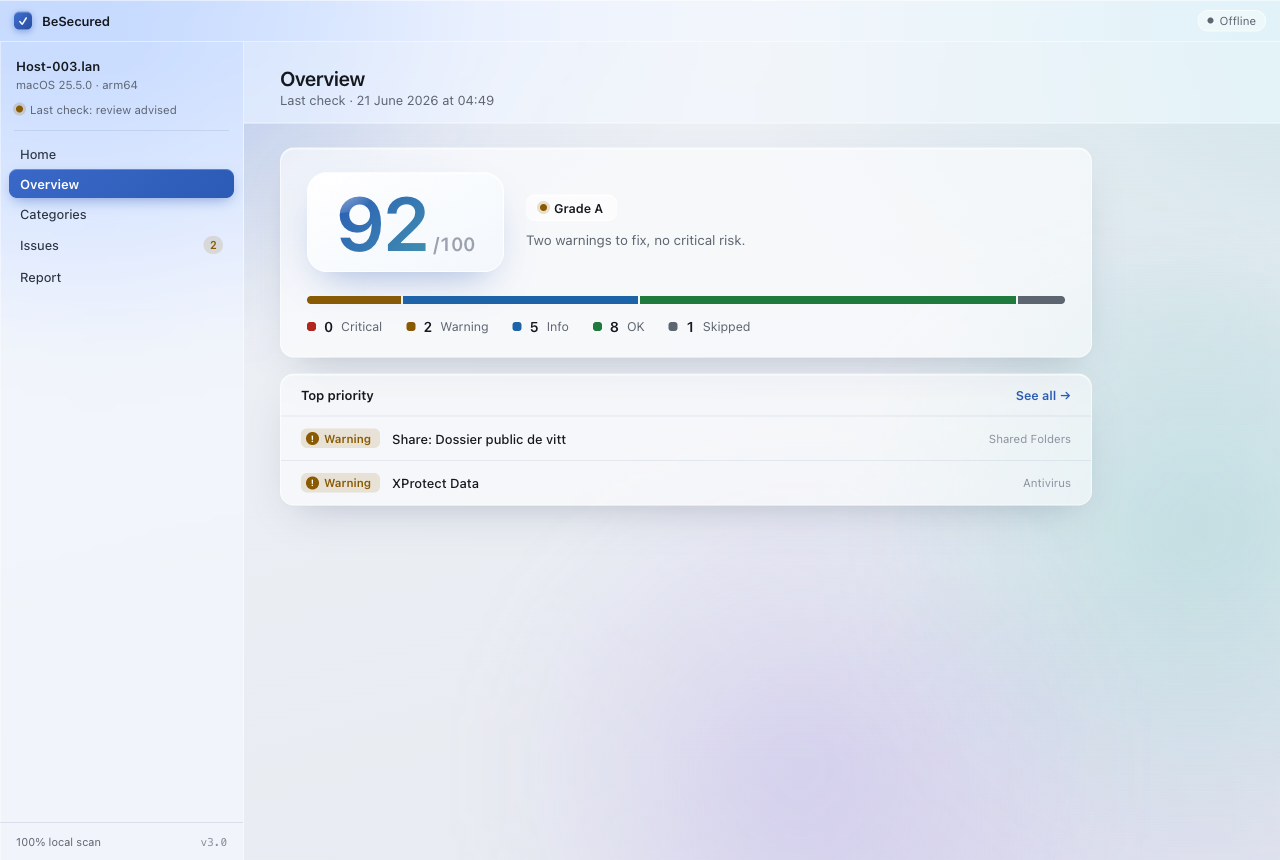
\includegraphics[width=0.82\linewidth]{ui-overview.png}
\caption{Overview after a scan: the score out of 100, the grade, and the breakdown by
status, on the local machine.}
\label{fig:overview}
\end{figure}

\section{Privacy}

Nothing leaves the machine. There is no account and no server to talk to: the interface
listens on 127.0.0.1 and the scan is local. Reports are written to a local folder, and
the program refuses to save one onto a cloud-synced path such as iCloud, OneDrive or
Dropbox, so a report cannot leave the device by accident. A test checks that the
interface files contain no external link, which keeps the promise honest as the code
changes.

\section{Testing}

The project has 96 automated tests, up from 59 in the previous report. They cover:

\begin{itemize}
\item the parsers and checks for each operating system;
\item the dispatch to the right OS module;
\item the scoring, the grades and the calculation steps;
\item the HTML and JSON export;
\item the JSON contract between the scanner and the interface;
\item the local scan endpoint;
\item a guard that the interface holds no remote reference.
\end{itemize}

They all pass. The suite runs with \texttt{python -m unittest discover -s tests}.

\section{Risks and what is left}

\begin{table}[h]
\centering\small
\begin{tabular}{@{}p{0.30\linewidth}p{0.62\linewidth}@{}}
\toprule
Risk & How we handle it \\
\midrule
Some checks need admin rights & Detected at runtime; the check is skipped with a note instead of failing. \\
False positives could mislead a non-expert & Unavailable checks are skipped, not passed; the result shape is guarded by tests. \\
Sensitive data must stay local & Local-only design, 127.0.0.1, the cloud-path guard, and a test for external links. \\
The optional AI part could slip & It stays optional and gets dropped first if week 8 or 9 runs late. \\
\bottomrule
\end{tabular}
\end{table}

What is left is short. Week 8: package the app for Windows and macOS so it opens with a
double click, run the full test pass, and do a last privacy check. Week 9: the optional
plain-language explanations for the top findings, generated locally if we can. Week 10:
the demo, the documentation and the handoff. The base is solid, so the remaining work
is about packaging and polish rather than new features.

\end{document}
